\documentclass{article}

\author{Tran Van Tan Khoi}

\date{May 20, 2025}

\title{Weekly Homework Report \#7}

\usepackage[utf8]{inputenc}
\usepackage[a4paper,top=2cm,bottom=2cm,left=3cm,right=3cm,marginparwidth=1.75cm]{geometry}
\usepackage[colorlinks=true, allcolors=blue]{hyperref}
\usepackage{graphicx}

\begin{document}

\maketitle

\section{Introduction}
\label{introduction}

I present my implementation of insertion, removal, and other functions of the binary tree, binary search tree, and AVL tree. These are not properly tested, but should work in theory. The source code is available on \href{https://github.com/xtrkoi/throwaway-rep}{Github}.

\begin{figure*}[h]
    \centering
    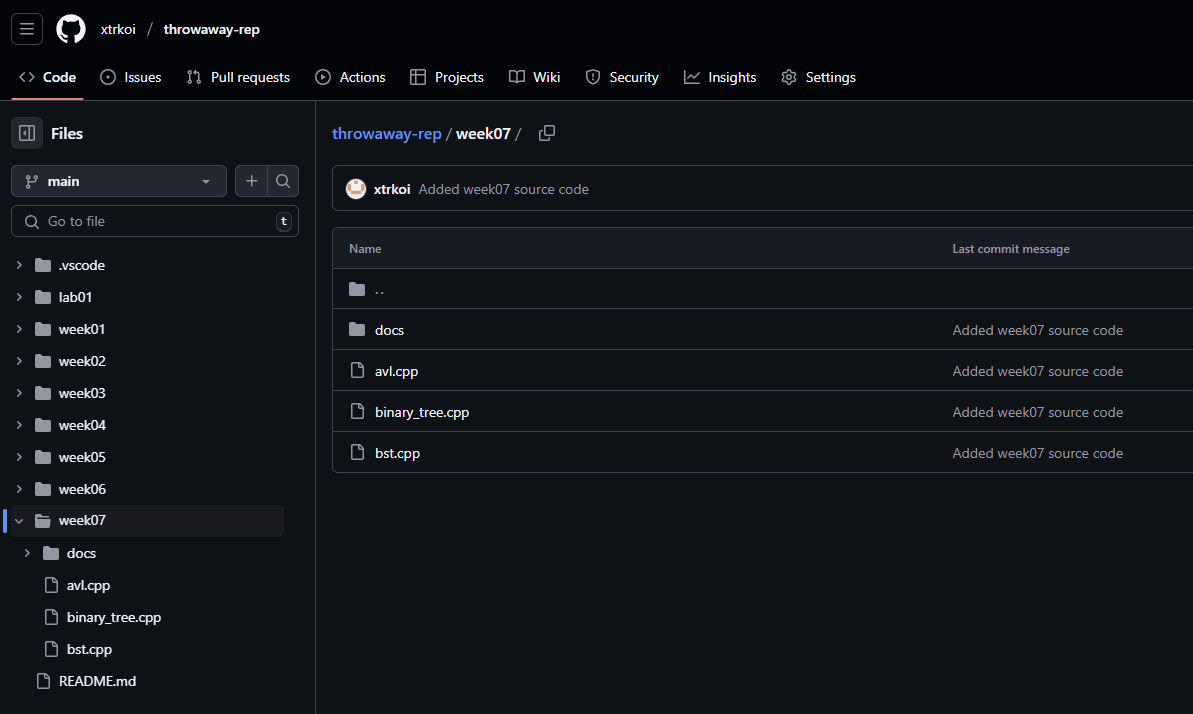
\includegraphics[width=12cm]{images/github_page.png}
\end{figure*}


\section{Binary Tree}
\label{binary_tree}

A \emph{tree} is a non-linear data structure consists of nodes connected by edges. All nodes in a tree are connected and the path connecting any pair of nodes is uniquely determined. A node in the tree will be chosen as the \emph{root}. For each node, the neighboring nodes that is farther away from the root are called its \emph{children}, and the neighboring node closer to the root is called the \emph{parent}.

\emph{Binary Tree} is a tree in which each node has at most two children. Going up the tree is travelling to the parent of the node, and going down is to one of the children. The root has no parent, the \emph{leaves} has no children (which can also be the root if the tree only has the root) and \emph{ancestors} are nodes we can move to by going up the tree. The \emph{subtree} of a given node is a tree with without any nodes or edges that can't be travelled to by going down the tree from the given node.

\subsection*{Traversal}
\label{traversal}

There are 3 types of traveral in a binary tree: \emph{Pre-order}, \emph{In-order}, and \emph{Post-order}. In each type of traversal, we start at the root, travel into the left subtree, then the right subtree. The moment we record and process the current node differentiate the type of traversal. Process the current node first would make the traversal pre-order. Doing so in between the subtrees would make the traversal be in-order. And after traversing both subtrees, it would be post-order traversal.

\subsection*{Level and Height}

For a given node, its \emph{level} is the distance between the node and the root, with the root having level 0. The height of a node is the maximum distance between the node and a leaf in its subtree, with all leaves in the tree having height 0.

\section{Binary Search Tree}
\label{binary_search_tree}

A \emph{Binary Search Tree} is a tree with the property: each node in the left subtree has a lesser value than the current node's value, and each node the right subtree has a greater value the the current node's value. This allows us to \emph{search} for a node with given value in the tree by making a binary decision at each node. To search for the node with given value, starting at the root, we will stop if we are sitting at the appropriate node, move down into the left subtree if the value we are looking for is less than the value in the current node, and into the right subtree if it is the opposite.

\subsection*{Insertion and Deletion}
\label{bst_insertion_deletion}

To make insertions and deletions in a binary search tree, we keep track of the left child and right child of each node individually.

To make insertions, we move down the tree the same way as we would search for a value and insertion a new node with the new value as a child of the node without the appropriate left child or right child.

Deletions are trickier. If the the node with the value to be deleted is a leaf node or only has one child, we can simply remove the node and connect the child to the parent, if the node has any. However, if the node has both children, the solution is to replace the value of the node with the value of the \emph{successor} (or \emph{predecessor}) node in the tree, and remove the successor (or predecessor) node in the tree. The successor (or predecessor) node is the node with the smallest (or greatest) value greater than (or less than) the current node's value. It can be proven that this node will always be a leaf node, and the removal of a leaf node can easily be handled.

\section{AVL Tree}
\label{avl_tree}

Realistically, insertion, deletion, and search operations on a binary search tree should take $O(h)$ time complexity, where $h$ is the height of the tree (which is the height of the root node). However, denoting $n$ as the number of nodes in the tree, the operations can take at most $O(n)$ if each node in the tree only has one child, creating a long connecting path of nodes, which is not ideal. To remedy this, we take into account the \emph{balance} of each node and make \emph{rotations} at unbalanced nodes so the the height of the tree is consistently $h \approx \log n$, so the time complexity of the common operations are $O(\log n)$.

\emph{AVL Tree} is a type of \emph{Balanced Binary Search Tree}, where after each insertion or removal, the search tree balances itself so the height of the tree is always approximately $\log n$.

\subsection*{Tree Balance and Rotations}
\label{balance_and_rotations}

Each node in an AVL tree maintains a \emph{balance factor}, defined as the difference between the heights of its left and right subtrees. Formally, for a node $v$, the balance factor is $BF(v) = h(v_L) - h(v_R)$. In an AVL tree, the balance factor of every node must be $-1$, $0$, or $1$. If an insertion or deletion causes the balance factor of any node to fall outside this range, the tree must be rebalanced.

Rebalancing is performed using \emph{rotations}, which are local restructuring operations that restore the AVL property. There are four types of rotations:
\begin{itemize}
    \item \textbf{Right Rotation (LL case):} Applied when a node's left subtree is heavier due to an insertion in the left child's left subtree.
    \item \textbf{Left Rotation (RR case):} Applied when a node's right subtree is heavier due to an insertion in the right child's right subtree.
    \item \textbf{Left-Right Rotation (LR case):} Applied when a node's left subtree is heavier due to an insertion in the left child's right subtree. This is a combination of a left rotation on the left child followed by a right rotation on the node.
    \item \textbf{Right-Left Rotation (RL case):} Applied when a node's right subtree is heavier due to an insertion in the right child's left subtree. This is a combination of a right rotation on the right child followed by a left rotation on the node.
\end{itemize}

These rotations ensure that after each insertion or deletion, the AVL property is restored and the tree remains balanced.

\subsection*{Insertions and Deletions in AVL Tree}
\label{avl_insertion_deletion}

Insertions and deletions in an AVL tree are performed similarly to those in a standard binary search tree. However, after each insertion or deletion, we must check all ancestors of the affected node for balance and make rotations if necessary.

After inserting a new node as in a binary search tree, we traverse up the tree from the inserted node, updating the heights and balance factors of each ancestor. If an ancestor becomes unbalanced, we identify the case (LL, RR, LR, or RL) and perform the corresponding rotations to rebalance the tree. Only the lowest unbalanced ancestor needs to be rebalanced after an insertion.

After deleting a node, we similarly traverse up from the parent of the deleted node, updating heights and balance factors. If any ancestor becomes unbalanced, we perform the necessary rotations. Unlike insertion, multiple ancestors may require rebalancing after a deletion, so we continue checking up to the root.

These rebalancing steps ensure that the height of the AVL tree remains $O(\log n)$, guaranteeing efficient search, insertion, and deletion operations.

\section{Conclusion}
\label{conclusion}

We can see the development of capabilities from just storing data in a binary tree, to adding searching functionality the binary tree, to maintaining efficiency of common operations on such trees using tree rotation and rebalancing. This proves to be useful in keeping ordered data, much like the \emph{set} container in C++'s Standard Template Library (STL).

\end{document}